\section{Framework to Develop Certifiable Pipeline Algorithms}
\label{sec:fundamental-tasks}

We have developed a framework of three pipelining primitives to create certifiable pipeline algorithms. The key to our approach is the observation that these primitives are 
%that have the potential to change the execution flow. There may be other optimizations, but these primitives 
both necessary and sufficient to create a simple pipeline from an unrolled loop in behavioral synthesis. If we can certify these primitives individually, we can build on them to create a certifiable pipelining algorithm.

\begin{figure}[t!]
\begin{center}
\begin{tabular}{cccc}
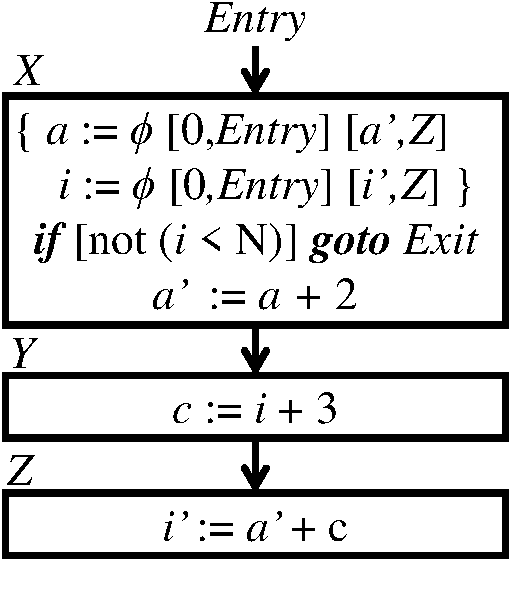
\includegraphics[height=1.4in]{fig-rpe/one-iteration-of-loop}
&
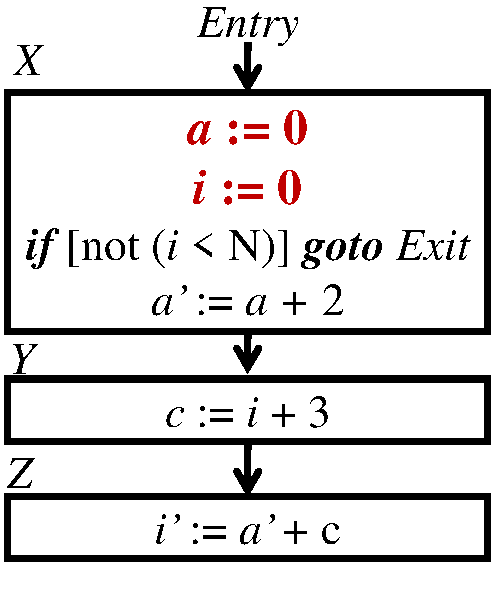
\includegraphics[height=1.4in]{fig-rpe/phi-removal-transformation}
&
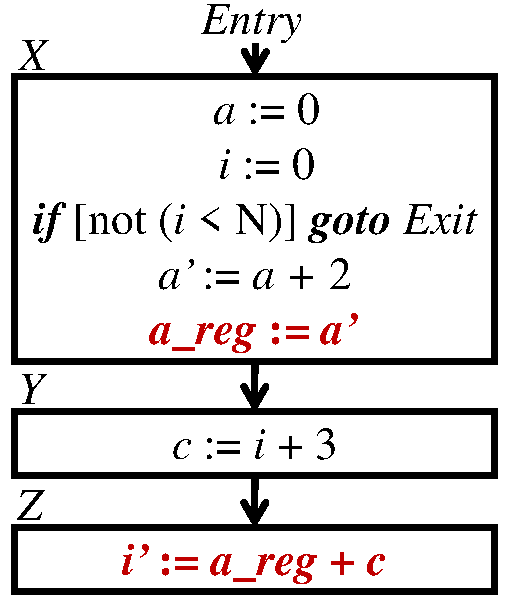
\includegraphics[height=1.4in]{fig-rpe/shadow-register-transformation}
&
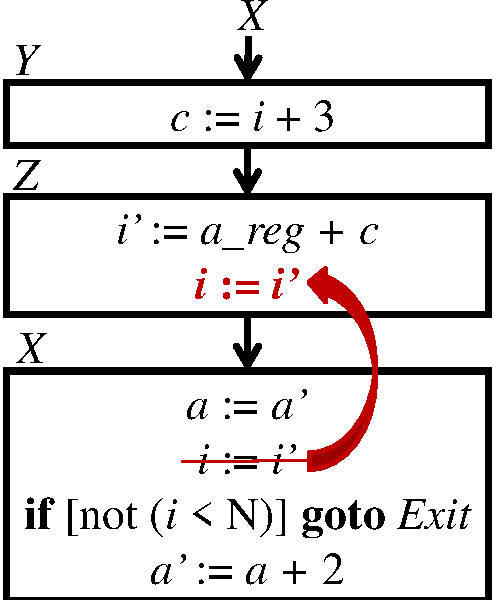
\includegraphics[height=1.4in]{fig-rpe/interchange-transformation}
\\
(a) & (b) & (c) & (d)
\end{tabular}
\end{center}
\caption{(a) First iteration of a loop (b) After $\phi$-elimination primitive (c) After shadow register primitive (d) After interchange primitive}
\label{fig:fundamental-steps}
\end{figure}

\begin{enumerate}
\item \textbf{\emph{$\phi$-Elimination Primitive}}: As mentioned earlier, a $\phi$-construct is a list of $\phi$-statements.
A $\phi$-statement is $v := \phi [\sigma, X] [\tau, Y] $, it executes as $ v := \sigma$ if the statement is reached from $X$ and as $ v := \tau$ if the statement is reached from $Y$. In figure~\ref{fig:fundamental-steps}(b), $i$ gets assigned the value $0$ as the scheduling step before the $\phi$-statement in the first iteration is $Entry$. A $\phi$-statement is used extensively in loops to perform different actions depending on whether the loop body is executed the first time. 

Reasoning about $\phi$-statement is complex since the state depends not only on $s$ but also on the previous scheduling step in the execution history after its execution from state $s$. However, 
we only deal with loops which do not have branching between the scheduling steps. Hence, if we unroll the loop, we can clearly identify a $\phi$-statement and its previous scheduling step in the execution history. So, we can convert each $\phi$-statement to its corresponding assignment statement based on the previous scheduling step in the unrolled loop structure. This primitive is called $\phi$-elimination primitive {\em i.e.,} given the previous scheduling step in the execution history, replace a $\phi$-construct with a list of corresponding assignment statements. 
\begin{gather*}
\{   a := \phi [0, Entry] [a', Z] \\ 
     \,\,\,\,\,\,i := \phi [0, Entry] [i', Z]   \} 
\end{gather*}
The $\phi$-construct given above is replaced with assignment statements given below in Figure~\ref{fig:fundamental-steps}(b).
\begin{gather*}
a := 0 \\
i := 0  
\end{gather*}

\medskip
\item \textbf{\emph{Shadow Register Primitive}}: If a variable $x$ is written in some microstep, then the shadow register primitive allows us to insert a shadow register step after this microstep. A shadow register step is basically the following assignment instruction: 
$$x\_reg := x$$ 
In the shadow register step here, $x\_reg$ is a new shadow variable introduced by the primitive (not part of the state in the original sequential loop). Now, since both $x$ and $x\_reg$ have the same value, the primitive replaces all subsequent reads of $x$ with $x\_reg$ till the next write of $x$. Suppose, the state before executing this step is $s_1$ and after executing is $s_2$, then we have the following relation:

$$ s_2 := s_1 \cup \{ \langle x\_reg, V \rangle \mid V  \text{ is the value of } \allowbreak  x \text{ in } s_1\} $$

As a result, the state with respect to real variables (all variables except shadow registers) is still $s_1$. 
In Figure~\ref{fig:fundamental-steps}(c), we have applied the shadow register primitive to the following microstep: 
$$a' := a + 2$$
We add a shadow register step: 
$$a\_reg := a'$$ 
We then replace the read of $a'$ in $Z$ with $a\_reg$. Note, since we know how each statement executes, we can identify the variables read and written in a statement statically.

\medskip
\item \textbf{\emph{Interchange Primitive}}: If two adjacent microsteps $m$ and $n$ are such that if a variable is written in $m$, it is not read or written in $n$ and vice versa, then we can move $n$ before $m$ without affecting the execution. Also, we can change the scheduling step of a microstep if the order of execution of the microsteps in the CCDFG remains same. In Figure~\ref{fig:fundamental-steps}(d),  
$i := i'$ is first interchanged with $a := a'$ since there is no read-write conflict between the two microsteps. Then, we rearrange the microstep $i := i'$ by moving it from $X$ to $Z$ without affecting the sequence of microsteps. Interchange does not work on microsteps which have a conditional branch statement. We will extend interchange primitive to include these statements in future.

\end{enumerate}
%\item \emph{Superstep construction} -- This operation entails combining the scheduling steps of the successive iterations, forming scheduling ``supersteps'' that act as scheduling steps for the pipelined implementation.  The result for our example is shown in
%Figure~\ref{fig:correctness}(c).  Supersteps must
%account for read-after-write hazards, i.e, if a variable is written in a scheduling step $X$ and read subsequently in
%$Z$ then $Z$ cannot be in a superstep that precedes $X$ in the control/data flow.  Note that we implement data forwarding (forward value of data within a single clock cycle); thus $X$ and $Z$ can be in a single superstep.


	
%\medskip
%\subsection{An ongoing proof of the correctness criterion}
%\label{sec:proof}	
%Our correctness statement naturally breaks into correctness of $\phi$-elimination, shadow register insertion, and superstep construction.
%The $\phi$-elimination theorem reduces to showing that our
%algorithm correctly replaces $\phi$-statements with
%assignments.  Note that this is not trivial since the algorithm has to use static analysis to
%deduce the previous basic block.  Correctness of shadow
%registers requires verifying similar static
%analysis (\eg, to determine the subsequent read of a
%variable after each write. For superstep construction, we need to verify that we can interchange any two adjacent steps which do not have any data dependencies or read-write conflict by static analysis. A series of interchanges can result in a whole block being moved up to create pipeline. 


